\documentclass[a4paper,12pt]{report}

\usepackage{graphicx} 
\usepackage{indentfirst}
\usepackage[spanish]{babel}
\usepackage{subfig}
\usepackage{biblatex}
\addbibresource{biblio.bib}

\begin{document}

\title{Curso práctico multiplataforma de Tratamiento Digital de la Imagen con Jupyter}
\author{ Ana Cuevas Bravo}
\maketitle

\newpage
\pagenumbering{roman}

\renewcommand{\abstractname}{Resumen}
\renewcommand{\chaptername}{Capítulo}
\renewcommand{\chaptername}{Capítulo}

\begin{abstract}
Your abstract goes here...
...
\end{abstract}


\tableofcontents
\newpage
\pagenumbering{arabic}

\chapter{Introducción}
\chapter{Objetivos}
\section{Objetivos}
\section{Requisitos}
\section{Metodología}
\chapter{Infraestructura}

En esta sección se detallan tanto el software empleado para la realización del trabajo, como la estructura previa que existía en la asignatura y que ha servido como base para las nuevas prácticas. \\

 El lenguaje de programación utilizado ha sido Python. Profundizaremos en las bibliotecas que tiene este lenguaje para el tratamiento de imagen que han sido necesarias para el desarrollo del trabajo. Esta sección también explicará en que consiste la plataforma Jupyter Notebook y las ventajas que tiene en su uso para la docencia. Por último, se hablará de Matlab, la plataforma original que se usa en la asignatura de Tratamiento Digital de la Imagen y la estructura general que tienen las prácticas de esta asignatura.

\section{Python tratamiento de imagen y visualización}

Python es un lenguaje de programación interpretado de alto nivel orientado a objetos, creado en los años 80 por Guido van Rossum. Se caracteriza por tener una sintaxis sencilla, fácil de leer, lo que facilita el mantenimiento de programas y lo hace accesible para principiantes. Tiene una amplia biblioteca base y además permite el uso de módulos y paquetes. Al ser interpretado en lugar de compilado el proceso de depuración es más rápido. En este trabajo se ha usado la versión 3.7.4 de Python.\\

 Python se está usando cada día más para el tratamiento de imagen, esto se debe a que es un lenguaje muy accesible, siendo gratuito y con una sintaxis sencilla. Con el tiempo han ido surgiendo bibliotecas específicas para el tratamiento de la imagen en Python como Pil (Python Imaging Library) también llamada Pillow, Scikit-image y Open-CV. Esta última será la que más se use en este proyecto.\\

Otra biblioteca que facilita el tratamiento de imagen en Python es Numpy, una biblioteca para facilitar el uso de matrices y arrays en Python, así como las funciones matemáticas relacionadas.  Además, Matplotlib que permite  la representación de datos en forma de gráficos.

\subsection{OpenCV}

OpenCV(Open Source Computer Vision Library) es una biblioteca centrada en el tratamiento de imagen y video (Computer Vision) y en aprendizaje de máquina, con interfaces para varios lenguajes de programación como C++, Python o Java. OpenCV es la biblioteca de procesamiento de imagen más usada en el mundo con más de 18 millones de descargas. Originalmente programada en C; el resto de lenguajes usa diferentes interfaces para acceder al código. Esto permitetener un buen rendimientopor ser C unl lenguaje muy rápido en ejecución.\\

OpenCV contiene  desde funciones de bajo nivel para el procesado de imagen hasta algoritmos complejos para deteccion de caras. En este trabajo, ya que trata de dar una base de tratamiento de imagen, usaremos funciones de bajo nivel como filtros o funciones para cambiar de espacio de color.\\

Se ha usado la versión 4.2.0 de OpenCV.\\


\subsection{Numpy}

Numpy es el paquete principal para cálculos complejos con matrices en Python, esto lo convierte en un paquete esencial en el desarrollo de código para usos ciéntificos y de robótica. La base de esta biblioteca es el objeto \emph{ndarray}, que consiste en arrays de n-dimensiones con datos de un mismo tipo y un tamaño establecido al crear la variable, esto último lo diferencia de las listas de python que son dinámicas.\\

En este trabajo se ha usado la versión 1.16.5 de Numpy.

Numpy contiene funciones que permiten realizar operaciones con grandes cantidades de datos de una forma más eficiente en memoria y rápida que usando las funciones propias de Python. Numpy está programado y pre-compilado en C. El uso de las funciones de Numpy también permite que el código se parezca más a la notación matématica estándar, lo que lo hace más fácil de leer y entender.\\

\subsection{Matplotlib}

Matplotlib es una biblioteca para la creación de gráficos en Python. También permite la representacion de imágenes. Matplotlib está construido usando Numpy para funcionar con el paquete general de Scipy. Permite interactúar con los gráficos de una forma muy similar a la representación de Matlab. Matplotlib funciona sobre cualquier sistema operativo. \\

Una de las razones por las que se ha elegido esta biblioteca para representar las diferentes imágenes y gráficos de las prácticas de TDI es por cómo interactúa con los cuadernillos de Jupyter, ya que permite la visualización de los gráficos incrustrada en el propio cuadernillo sin crear otra ventana. \\

Otro punto a favor de Matplotlib es la capacidad para interactuar con los gráficos, cómo ya se ha mencionado antes, esto es algo que permite Matlab e interesaba mantener en las prácticas, ya que puede ayudar mucho a la hora de entender algunos de los ejercicios. Esta interactividad consiste en la posibilidad de hacer zoom en los gráficos y un cursor que indica el valor del pixel sobre el que está.

Se ha usado la versión 3.1.1.\\

\subsection{Scikits}

Abreviatura de Scipy Toolkits son una serie de paquetes añadidos para scipy separados de su distribución principal. Estos paquetes se separan de scipy cuando se consideran demasiado específicos para el propio Scipy, por una licencia incompatible con la de Scipy o si aún están en desarrollo.\\

En este trabajo se van a usar 2 de esos kits:\\


\begin{itemize}

	\item \textbf{Scikit-learn}:es un paquete con un amplio rango de algoritmos de aprendizaje de máquina para problemas de tamaño medio, tanto supervisados como no supervisados. Está programado mayoritariamente en Python aunque incorpora algunas bibliotecas de C++ e incorpora código compilado para mejorar su eficiencia.

	\item \textbf{Scikit-image}:este paquete cuenta con una colección de algoritmos para el tratamiento de imagen construida por una comunidad de voluntarios.
\end{itemize}
\section{ Cuadernillos de Jupyter}

El cuadernillo Jupyter es una interfaz web de código libre, que permite la creación de documentos que contienen código ejecutable, ecuaciones, visualización (gráficos, imágenes) y texto. Trabajaremos sobre la versión \\

El cuadernillo se guarda como un JSON la extensión .ipnyb. La aplicación es un modelo cliente-servidor que se ejecuta a través de un navegador. Se trata de un servidor local que se crea al ejecutar la aplicación lo que implica que no se necesita conexión a internet para leer o modificar un cuadernillo.  El servidor lee el documento .ipnyb y manda mensajes usando ZeroMQ (una librería que manda mensajes usando un modelo asíncrono) a un kernel que ejecuta el código Python en el cuadernillo. El cliente funciona en un navegador y es lo que permite interactuar con el cuadernillo. Según se muestra en la figura \ref{estructurajupyter}
\begin{figure}[h]
\centering
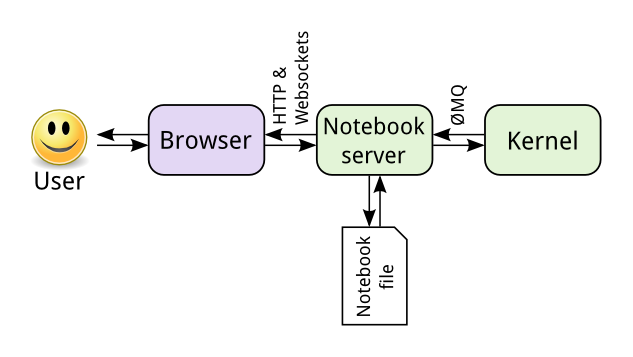
\includegraphics[width=1.0\textwidth]{imagenes/estructurajupyter}
\caption{Estructura de Jupyter Notebook.}
\label{estructurajupyter}
\end{figure}

Los cuadernillos de Jupyter consisten principalmente en dos tipos de celdas: \emph{code} y \emph{markdown}.\emph{ Code }son las celdas ejecutables en las que se escribe código de Python, mientras que \emph{markdown} son las celdas de texto. Para estilizar el texto se usa  la sintaxis de markdown, que permite desde poner texto en negrita hasta insertar imágenes o fórmulas matemáticas complejas.\\




\section{Prácticas de TDI en Matlab}


Las prácticas originales para la asignatura de Tratamiento Digital de la Imagen consisten en una carpeta zip que se pone a disposición de los alumnos en el aula virtual de la asignatura. Dentro de esta carpeta están las imágenes que se van a utilizar en la práctica (cuando no eran imágenes internas de MatLab), funciones adicionales necesarias en caso de que no existieran previamente y un enunciado en pdf. En la imagen \ref{carpetapracticas} se puede ver un ejemplo de una de estas carpetas.
 
\begin{figure}[h]
\centering
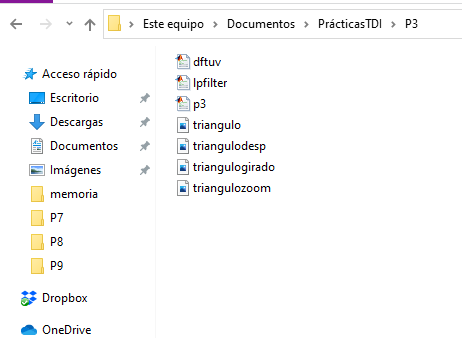
\includegraphics[width=0.5\textwidth]{imagenes/carpetapracticas}
\caption{Ejemplo de carpeta de prácticas.}
\label{carpetapracticas}
\end{figure}

Las prácticas se realizaban en hora de clase en uno de los laboratorios de Windows del campus. Se podían realizar enteras en la duración de la clase. \\

La profesora daba una breve explicación inicial sobre el tema de la práctica, siempre relacionado con lo que se hubiera dado en las clases de teoría recientes. El resto de la práctica se podía seguir de forma libre con el enunciado, con la profesora respondiendo las dudas que surgieran en el desarrollo del ejercicio. \\

Los enunciados son instrucciones detalladas sobre los pasos a seguir para realizar la práctica, con poco o nada de teoría, ya que se asume que el alumno ha recibido las clases de teoría previas. El alumno debe crear un nuevo documento en Matlab e ir ejecutando paso a paso lo que pide el enunciado. \\

Los enunciados suelen comenzar con un breve párrafo explicando el objetivo de la práctica. Por ejemplo en la práctica 4 que trata el tema de segmentación de Imagen, la introducción dice:\emph{``El objetivo de esta práctica es comenzar a familiarizar al alumno con las herramientas básicas de segmentación de imagen en entorno MATLAB. Para ello se trabajará con la imagen en escala de
grises ‘calculadora.tif’, que acompaña al material de esta práctica. "}\\

A partir de esta breve introducción la práctica suele estar dividida en secciones normalmente relacionadas con diferentes puntos tratados en la teoría y cómo llevarlos a cabo.\\

Los pasos a seguir en MatLab, por lo general, vienen dados en el enunciado que indica qué función usar y cómo llamar a las diferentes variables para mantener una consistencia en los nombres a lo largo de la práctica. En algunos casos se indican las variables necesarias para llamar a la función que se va a usar en esa sección del ejercicio, mientras que en otros se pide al alumno que use el comando \textsl{+help} para informarse sobre el funcionamiento de la función. Del mismo modo si una función requiere de un valor a decidir, dependiendo de lo que se quiera conseguir con su uso, unas veces se da con el enunciado y otras se deja a criterio del alumno para que pruebe cómo cambian los resultados con diferentes variables y cuál sería la mejor solución para el problema planteado.\\

Otra característica común de los enunciados de TDI son las preguntas para responder, aunque no se pide una memoria en sí de las prácticas en los enunciados hay preguntas con el objetivo de que el alumno se plantee las respuestas y las razones de los pasos que se han ido realizando durante el ejercicio.  La siguiente imagen \ref{preguntasp4} muestra un ejemplo de estas preguntas del principio de la práctica 4.

\begin{figure}[h]
\centering
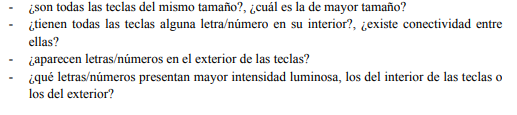
\includegraphics[width=1\textwidth]{imagenes/preguntasp4}
\caption{Ejemplo de preguntas realizadas en los enunciados de TDI.}
\label{preguntasp4}
\end{figure}

Algunos de los enunciados tienen imágenes del aspecto que tendría que tener la imagen sobre la que se está trabajando después de ciertos pasos para que el alumno pueda ver si el ejercicio progresa adecuadamente o si debería modificar alguna variable o revisar el código.\\

Si se pide un algoritmo un poco más complejo, en los enunciados aparece dado un trozo de ese código como ejemplo o directamente para copiar en Matlab ya que el objetivo de estas prácticas no era aprender a programar en MatLab sino ilustrar de forma práctica lo dado en teoría de la asignatura.\\

Las prácticas se suelen centrar en el tratamiento de una imagen en específico, elegida para ilustar el tema del que trata la práctica. Por ejemplo en la práctica 1, en el apartado que trata sobre color se escoge una imagen con diferentes verduras que muestran una variedad de colores para ilustrar la mezcla aditiva de color al representarse individualmente las matrices de cada color del sistema de representación RGB. Debido a que algunas de las imágenes usadas en las prácticas originales pertenecen a Matlab o se desconoce su origen se ha tenido que buscar imágenes nuevas, siempre intentando mantener las características de la imagen original.\\

En total la asignatura consiste de 9 prácticas, 7 de imagen y 2 de video. \\

\begin{itemize}
  \item [ P1.]\emph{Introducción al tratamiento de imagen:}\\
	Esta práctica es una introducción a las herramientas de tratamiento de imagen en Matlab. Se trata como leer y representar imágenes, espacios de color, escalado e histogramas. El último apartado se centra en imágenes RGB.
  \item [P2.]\emph{ Filtrado de imágenes en el dominio espacial:}\\
	Esta práctica demuestra el funcionamiento de diferentes tipos de filtros sobre imágenes contaminadas con varios ruidos. En la segunda parte se tratan filtros de realce de contorno y se demuestra su uso para para extraerlos bordes de unas monedas.
  \item [P3.]\emph{Filtrado de imágenes en el dominio espectral:}\\
	En esta práctica se demuestran las propiedades de la transformada de Fourier y como afectan las transformaciones en el espacio a la representación en frecuencia de la imagen. También se tratan filtros en el dominio frecuencial.
  \item [P4.]\emph{Segmentación de image:}\\
	Esta práctica es diferente a las anteriores ya que en lugar de ejercicios individuales se centra en el tratamiendo de una imagen en concreto con un objetivo claro. Se trata  la imagen de una calculadora con el objetivo de conseguir una nueva imagen en la que solo se vea la letra Enter de la calculadora. Para esto se usa segmentación binaria que es el tema de la asignatura que se corresponde con esta práctica.
  \item [P5.]\emph{Segmentación de imagen II:}\\
	Esta prácctica sigue el esquema de la anterior centrándose en la segmentación de una imagen, en este caso un pájaro. Para la segmentación de este pájaro se va a usar aprendizaje de máquina, específicamente el algoritmo K-medias, la mayor parte de la práctica se centra en en realizar diferentes transformaciones sobre la imagen para facilitar el uso del algoritmo.Entre estas transformaciones se encuentran cambios de espacio de color y filtros de textura.
  \item [P6.]\emph{Morfología binaria:}\\
	Este ejercicio aplica operaciones de morfología matemática para segmentar los chips de una placa y separarlos de acuerdo a su forma.
  \item [P7.]\emph{Segmentación opr watershed:}\\
	El objetivo de esta práctica es segmentar una imagen con células para contarlas. Para conseguir esto se plantea el uso del algoritmo de watershed con arcadores. Primero se extraen los marcadores internos de las células usando herramientas como la reconstrucción morfológica y conseguir los máximos regionales de una imagen, operaciones estudiadas en la parte correspondiente a esta práctica del temario, lo mismo ocurre con los marcadores exteriores y el uso de la transformada de distancia. Esta práctica además tiene el objetivo de demostrar que la segmentación de este tipo de elementos que muchas veces se encuentran superpuestos en a imagen es muy complicada y siguen dando bastante error.
  \item [P8]\emph{Manejo de vídeos en MATLAB. Detección y estimación de movimiento:}\\
	Esta es la primera de las prácticas de video, está dividida en dos secciones claras. La primera es una introducción a las herramientas de video en Matlab, estructura de video, como reproducir y guardar videos. La segunda parte trata 3 algoritmos de estimación de movimiento: EBMA, HBMA y correlación de fase.
  \item [P9]\emph{Mejora y restauración de vídeo. Filtrado interframe:}\\
	La segunda práctica de vídeo y la última de la asignatura trata la restauración de video contaminado con ruido de una forma muy similar a la práctica 2 de imagen. Primero se centra en el filtrado frame a frame y después en el filtrado interframe, es decir usando varios frames para compararlos entre si y así filtrar.
\end{itemize}

\chapter{Prácticas de TDI}

Este apartado tratará el desarrollo del proyecto, se irá analizando cada práctica de la asignatura y comparando la versión original con el resultado final en Python, se tratarán los diferentes problemas que han ido surgiendo a la hora de adaptar cada práctica y cómo se han solucionado.\\

\section{Estructura de las prácticas en Jupyter Notebook}

A la hora de plantear las prácticas en los cuadernillos de Jupyter lo primero que se hizo fue decidir que partes se iban a mantener igual y en qué se iban a diferenciar de las de Matlab. La estructura en si, el temario tratado, el orden de los ejercicios y en los casos que se podía las imagenes originales se intentan mantener intactas. Los más importante erra mantener el cometido de la práctica, lo que se pretendía mostrar y enseñar con ella.\\

El cambio más obvio entre las dos versiones de los ejercicios tiene que ver con los enunciados, en los cuadernillos el enunciado está en inglés ya que se había planteado el TFG para subir las prácticas a Robotics Academy, esto las haría más accesible a un mayor número de personas. Otro cambio en los enunciados es que han sido ampliados, esto se debe a que las prácticas originales son un material que se apoya sobre la teoría dada en clase y asumen que esa teoría ha sido impartida, mientras que en Robotics Academy las prácticas serían el único contacto que tendría el alumno con el tema por los que los nuevos enunciados amplian un poco las explicaciones teóricas añadiendo enlaces a más recursos para ampliar conocimientos.\\

Una cosa común en los enunciados originales son los trozos de código facilitados para copiar y pegar, en jupyter estas lineas de código apaercen en celdas tipo \emph{code} con indicaciones para cambiar los nombres de las variables si es necesario.\\

En cuanto al desarrollo de los ejercicos el cambio principal es el lenguaje de programación, de Matlab a Python. \\

Un cambio significativo en la presentación de la práctica es el uso de ventanas emergentes, cuando ejecutas las prácticas en Matlab con la cantidad de imágenes que se pide representar pueden aparecer hasta 20 pestañas nuevas  (imagen \ref{ventanas}) lo que puede ser bastante abrumador, en la versión desarrollada en este trabajo se han intentado evitar las ventanas emergentes, representando siempre que se ha podido en el propio cuadernillo, esto también hace las prácticas más fáciles de consultar una vez se ha terminado el código ya que se puede guardar el cuadernillo una vez ejecutado y las imágenes se mantienen mientras no se vacíe el output.\\

\begin{figure}[h]
\centering
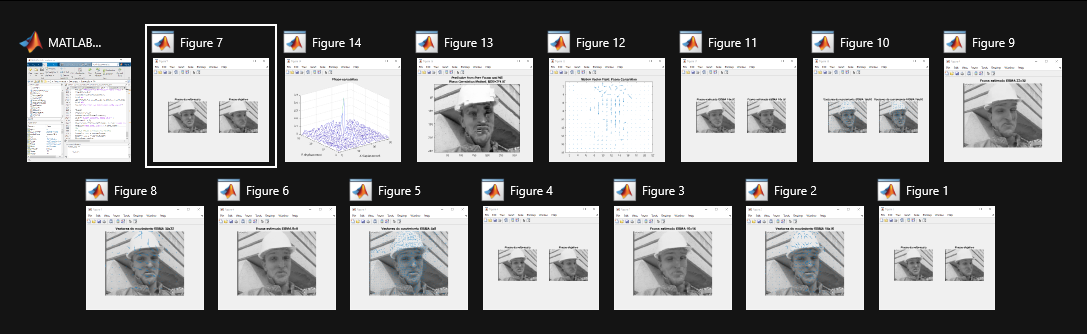
\includegraphics[width=1\textwidth]{imagenes/ventanas}
\caption{Ventanas emerjentes en el apartado 2 de la práctica 8 en Matlab.}
\label{ventanas}
\end{figure}

Por último, en los cuadernillos se ha añadido un nuevo apartado donde se muestra el aspecto que tiene que tener la imagen resultante de algunos apartados de la práctica. En una clase práctica de TDI siempre estaba la profesora, esto permitía que en caso de duda se le pudiese preguntar si iba bien la práctica enseñando la imagen resultado de un apartado en el que se tuviera duda. Las imágenes respuesta pretenden sustituir esta opción para los alumnos que accedan a las prácticas fuera del contexto de la asignatura de TDI.


\section{Guía de instalación}

Para facilitar el acceso a las prácticas se ha creado una guía de instalación en \emph{markdown} directamente accesible en Github desde el repositorio en el que están la prácticas.\\

La guía requiere que primero se compruebe si el ordenador tiene instalado Python3, en caso negativo, se pone un link a la página oficial de Python con la guía de instalación para los diferentes sistemas operativos.\\

A continuación, se indica como instalar Pip, el instalador de paquetes en Python y se indica el comando para instalar pipenv.\\

La guía continúa explicando cómo acceder a la prácticas y como iniciar el entorno de Pipenv necesario para ejecutarlas.\\

Por último, se explica como abrir un cuadernillo de Jupyter importando las librerías necesarias en la primera práctica para comprobar que el entorno se ha instalado correctamente.\\

Esta guía está en inglés, al igual que las prácticas y pensada para ser usada y funcionar por igual en cualquiera de los principales sistemas operativos. Ha sido probada en Windous y Linux Ubuntu.\\

\section{ Práctica 1: Introducción}

\subsection{Teoría tratada en la práctica}

En esta práctica se opera sobre la matriz de la imagen, también se explica de forma práctica la diferencia entre una imagen true color y una imagen indexada. Se pone un énfasis especial en los diferentes tipos de datos en matrices (double, uint64, float...) ya que a la hora de operar puede dar lugar a error.\\

El siguiente punto de la práctica se centra en la conversión de imágenes de color a gris y binario. A continuación se usan diferentes métodos para modificar la resolución de una imagen actuando tanto sobre la resolución espacial como la intensidad.\\

La práctica también explica cómo representar el histograma de una imagen y el efecto que tiene la ecualización del histograma sobre el contraste de la imagen.\\

Por último se verá la interpretación del color y cómo realizar transformaciones puntuales.\\

\subsection{Comparativa Matlab vs Python}

En este apartado vamos a mencionar las principales diferencias entre la práctica realizada en Matlab y el nuevo formato usando un cuadernillo de Jupyter.\\

En el primer apartado de la práctica que se centra en la lectura y representación de imágines podemos encontrar dos diferencias:\\

La primera es el espacio de color sobre el que se trabaja. Matlab y Matplotlib leen las imágenes de color como RGB mientras que OpenCV usa BGR, esto genera un conflicto entre la librería que se va a usar para leer imágenes y la que se va a usar para representar. Se resuelve en el siguiente apartado que trata sobre espacios de color.\\

La segunda son los métodos de representación. En Matlab teníamos una única funcion (\textbf{imshow}) que crea una ventana nueva con la imagen representada y herramientas como un cursor y la posibilidad de hacer zoom. En Pyhton tenemos dos opciones de representación, una es \textbf{imshow} en la biblioteca  OpenCv que al igual que Matlab genera una ventana nueva fuera del cuadernillo pero no tiene herramientas y la otra es \textbf{imshow} en Matplotlib que permite visualizar la imagen en el propio cuadernillo y tiene las mismas herramientas que Matlab.\\

La siguiente gran diferencia entre los dos ejercicios es en el apartado de conversión de tipos de imágenes. Como ya se mencionó, se ha añadido una transformación de espacios de color para solucionar el problema de lectura, pero la mayor diferencia tiene que ver con la falta de una función que convierta una imgen RGB a indexada que si exite en Matlab. Se probó a programar una versión equivalente en Python pero por cuestión de velocidad en la ejecución no se pudo implementar. El problema se solventó exportando las dos matrices que forman una imagen indexada desde Matlab  e implementarlas en Python aprovechando para explicar como se crean los mapas de color.\\

La falta de la función RGB2ind vuelve a ser relevante en el punto sobre modificación de la resolución de intensidad de una imagen, ya que en la práctica original se usaba esta función para cambier el número de niveles de intensidad en el mapa de color. Se resuelve explicando una resolución matemática al problema sin cambiar la imagen a indexada. Al ser una imagen en escala de grises con menos información que una imagen RGB también se puede usar la versión de Python de RGB2ind ya que el tiempo de ejecución es menor para imágenes en escala de grises. En la siguiente imagen \ref{resmatematica} se puede ver la parte del enunciado en la que se explica la resolución matemática. 

\begin{figure}[h]
\centering
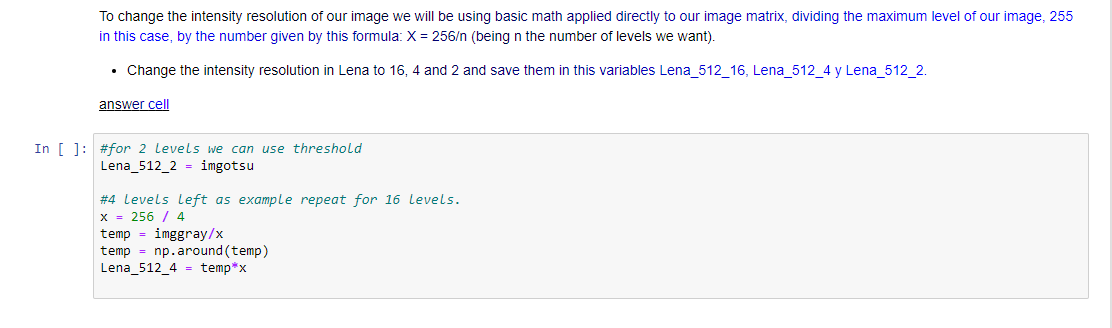
\includegraphics[width=1\textwidth]{imagenes/resolucionmatematica}
\caption{enunciado del apartado sobre resolución de intensidad}
\label{resmatematica}
\end{figure}

En el apartado sobre el histograma, el único cambio, es la imagen utilizada para ejemplificar la ecualización del histograma ya que la imagen original pertenece a Matlab. Sucede lo mismo en el último apartado con la imagen de los pimientos.\\

Por último, en los cuadernillos se ha añadido un nuevo apartado donde se muestra el aspecto que tiene que tener la imagen resultante de algunos apartados de la práctica.

\subsection{Desarrollo de funciones}

En esta práctica solamente fue necesario desarrollar una función nueva: RGB2ind. Esta función se usa para convertir una imagen true color RGB en una imagen indexada con el número de niveles como parámetro. \\

A la hora del desarrollo se intentó buscar el código de la función original de Matlab pero, es de las funciones precompiladas en C y su código no es accesible. Se resolvió usando el algoritmo K-medias con un número de nucleos igual al número de niveles requeridos.\\

 La función final tiene un problema de tiempo de ejecución. Para un número pequeño de núcleos funciona bien pero, por ejemplo para los 256 requeridos en la práctica el tiempo de ejecución interrumpiría el desarrollo cómodo del ejercicio. Para mejorarla se podría probar a usar una versión pre-compilada de Python o programar la función en C e implementarla.\\

Esta imagen \ref{rgb2ind} muestra como queda la solución para una imagen indexada de 5 niveles.
\begin{figure}[h]
\centering
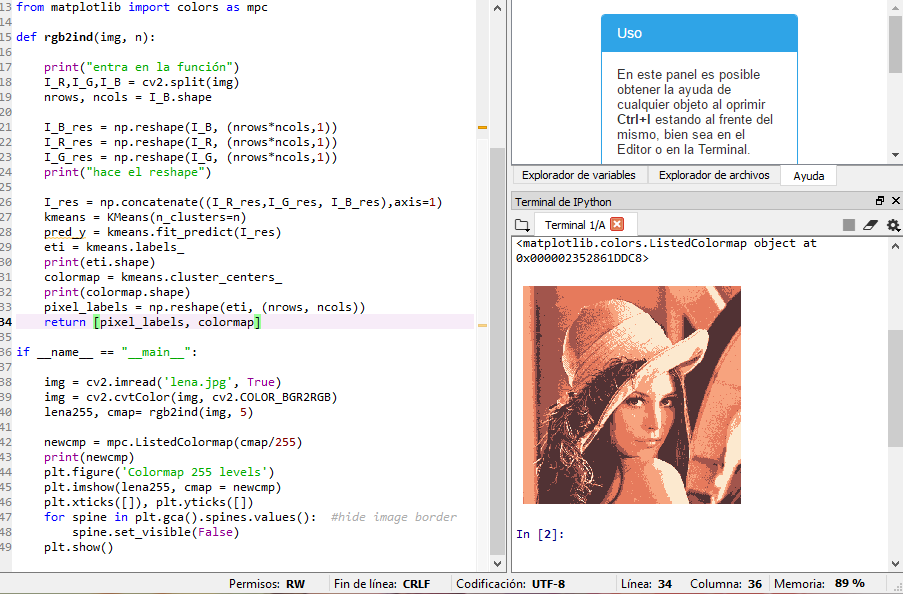
\includegraphics[width=1\textwidth]{imagenes/rgb2ind}
\caption{muestra de código y solución de RGB2ind}
\label{rgb2ind}
\end{figure}


\section{ Práctica 2: Filtrado espacial}

\subsection{Teoría tratada en la práctica}

Este segundo ejercicio se centra en el filtrado de imágenes en el espacio, se irán demostrando diferentes tipos de filtro y sus usos más comunes en la práctica.\\

El primer apartado enseña diferentes tipos de ruido y cómo contaminar una imagen, los tipos de ruido tratados son: ruido gaussiano, ruido de sal y pimienta y ruido granular.\\

Los filtros se dividen en dos categorías: filtros paso bajo y filtros paso alto. En esta práctica se explican dos filtros paso bajos diferentes. El primero es el filtro de media que es un filtro lineal. Consiste en ir colocando una máscara sobre la imagen y calculando la media de los píxeles bajo la máscara, este filtro genera un suavizado de la imagen [\ref{filtromedia}].

\begin{figure}[h]
\centering
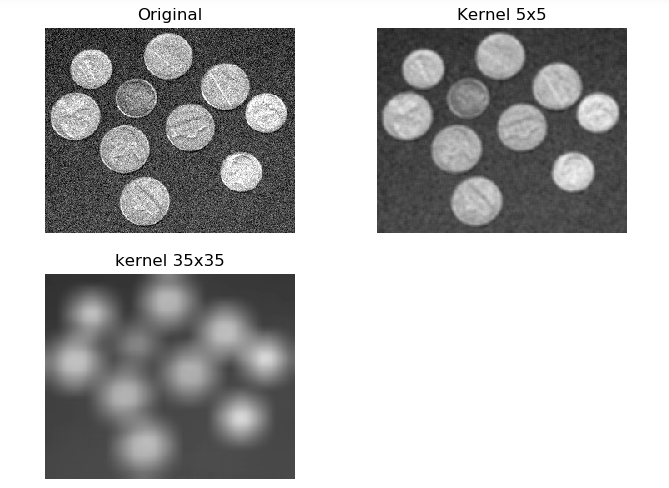
\includegraphics[width=1\textwidth]{imagenes/filtromedia}
\caption{imagen del cuadernillo donde se demuestra el filtro de media con diferentes tamaños de máscara}
\label{filtromedia}
\end{figure}

El otro filtro paso bajo es el filtro de mediana que es un filtro no lineal. Este filtro coge los valores de debajo de la máscara y  hace la mediana con esos valores, esto permite que se mantengan mejor los valores originales de la imagen, se usa para quitar ruido de sal y pimienta en la práctica.\\

Los filtros paso alto son filtros de realce de contornos. Se usan sobre todo para detectar bordes de objetos en la imagen. En esta práctica se dan dos tipos de filtro paso alto dependiendo de la máscara que usan: Prewitt e Isotrópico \ref{fpa}

\begin{figure}[!tbp]
  \centering
  \subfloat[Prewitt.]{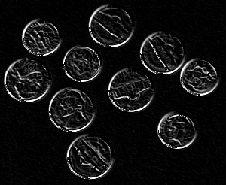
\includegraphics[width=0.4\textwidth]{imagenes/prewitt}\label{fig:f1}}
  \hfill
  \subfloat[Isotrópico.]{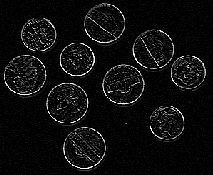
\includegraphics[width=0.4\textwidth]{imagenes/isotropic}\label{fig:f2}}
  \caption{Filtros paso alto.}
  \label{fpa}
\end{figure}

\subsection{Comparativa Matlab vs Python}

En el primer apartado de está práctica se usan una serie de funciones que no pertenecen a Matlab y vienen entre los materiales de la práctica, estas funciones se recrean en Python con la misma funcionalidad.\\

En el apartado de filtros lineales la función más importante es \textbf{imfilter} que tiene de parámetros de entrada la imagen a filtrar, la máscara y el tipo de \emph{padding}. El tipo de \emph{padding} indica como se va a rellenar la máscara cuando el valor del centro es un borde de la imagen, los dos tipos de \emph{padding} que se demuestran en esta práctica son \emph{zero padding} que rellena con 0 y \emph{mirror padding} que copia los píxeles cercanos al borde. La función \textbf{filter2D} de OpenCv funciona de la misma manera y con los mismos parámetros.\\

Es importante mencionar que para apreciar bien las diferencias de tipo de \emph{padding} se tienen que ver bien los bordes de la imagen. Matplotlib, por defecto, añade un borde negro a sus figuras, esto impide que se aprecie bien la diferencia. Se encuentra un comando adicional para quitar estos bordes por defecto.\\

Para el filtro de mediana también existe una función en OpenCV (\textbf{medianblur}) que funciona exactamente igual que el equivalente de Matlab.\\

La mayor diferencia en el apartado de realce de contornos la encontramos en la función \textbf{fspecial} de Matlab que genera máscaras específicas para los diferentes filtros paso alto. Esta función no existe en OpenCV, se usa Numpy para generar las matrices y se van metiendo los valores correctos de acuerdo con el tipo de filtro que se quiere usar. Para hacer el filtrado en sí, se usa la misma función que para los filtros lineales paso bajo.\\

El último apartado de composición de imágenes requiere funciones que se usaron ya en la práctica uno y una función nueva de Numpy para realizar sumas punto a punto de matrices de más de dos dimensiones. La solución final queda muy parecida a la original de Matlab.
\ref {p2final}\\


\begin{figure}[!tbp]
  \centering
  \subfloat[Matlab]{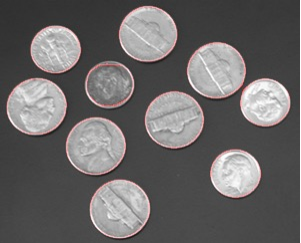
\includegraphics[width=0.4\textwidth]{imagenes/finp2ml}\label{fig:f1}}
  \hfill
  \subfloat[Python]{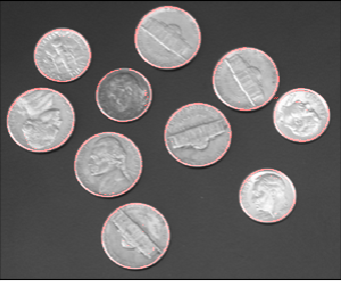
\includegraphics[width=0.4\textwidth]{imagenes/finp2py}\label{fig:f2}}
  \caption{Imágenes resultado del último aparatado de la práctica 2}
  \label{p2final}
\end{figure}


\subsection{Desarrollo de funciones}

Para este ejercicio se han tenido que desarrollar varias funciones, todas relacionadas con la función de añadir ruido en una imagen. La función principal \textbf{imnoise} tiene 3 parámetros de entrada: la imagen a contaminar, el tipo de ruido y un parámetro genérico que indica los parámetros de cálculo del ruido (por ejemplo si el ruido es gaussiano este parámetro contiene la media y la varianza). La imagen puede ser tanto en tonos de gris como en color. Para añadir el ruido se llama a \textbf{addnoise} que es la función que realiza las operaciones matemáticas necesarias.\\

Otras funciones que se han ido creando por necesidad de \textbf{imnoise} son \textbf{checkcolor} que, como su nombre indica, se encarga de comprobar si la imagen es de color y un par de funciones para cambiar el tipo de datos de la matriz de image,n por ejemplo, de unit8 a double y viceversa.

\section{Práctica 3: Filtrado en el dominio de la frecuencia}
\subsection{Teoría tratada en la práctica}

En esta práctica se trata la imagen en el dominio de la frecuencia. Se intenta mostrar de forma práctica cómo se ve una imagen en frecuencia y en qué consiste la transformada de Fourier bidimensional. Se explica porqué se necesitan dos representaciones diferentes para una misma imagen (módulo y fase) y qué representa cada una.\\

El segundo apartado demuestra las propiedades de la transformada de Fourier, qué transformaciones en el espacio afectan a la fase y cuáles al módulo y de qué manera.\\

El resto de la práctica se centra en el filtrado de imagen en el dominio frecuencial. Primero se explican dos filtros paso bajo: Gaussiano e ideal [\ref {gauss}]. Se trata de filtrar la imagen en frecuencia y ver como afecta en el espacio tras hacer una tranformada de fourier inversa.
\begin{figure}[h]
\centering
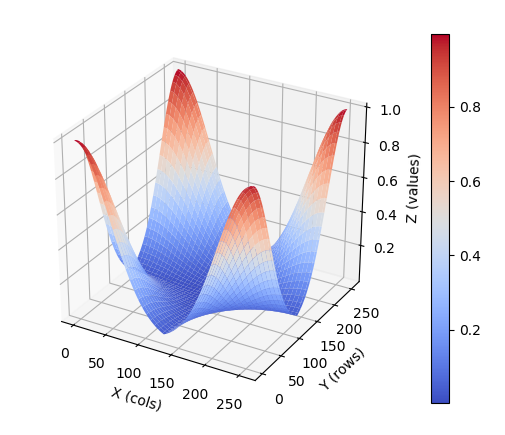
\includegraphics[width=0.6\textwidth]{imagenes/gaussfpb}
\caption{representación de un filtro paso bajo Guassiano}
\label{gauss}
\end{figure}
 Para concluir la práctica se tratan los filtros paso alto que, en el dominio de la frecuencia, son iguales que los filtros paso bajo pero invertidos.
\subsection{Comparativa Matlab vs Python}

En este ejercicio se usa una imagen dada con la práctica original de un triángulo blanco sobre un fondo negro.\\

La función más importante de esta práctica es \textbf{fft2}, la transformada de Fourier bidimensional. Existe un equivalente exacto en Numpy,  \textbf{numpy.fft.fft2}. También existe equivalente para la función \textbf{fftshift} que modifica la representación de la imagen en frecuencia para que las frecuencias bajas se concentren en el centro de la imagen y las altas en los extremos.\\

Para las representaciones en 3D se ha usado una función sacada de Github de código abierto, que simplifica el código de forma que, para representar un gráfico, solo tienes que llamar a una función en lugar de meter todas las especificaciones de Matplotlib cada vez que se quiera representar algo. En el cuadernillo se deja el código demostrando como usar esta función.\\

El apartado de propiedades de la transformada de Fourier se mantiene igual de Matlab a Python.\ref{zoom}\\

\begin{figure}[!tbp]
  \centering
  \subfloat[Matlab]{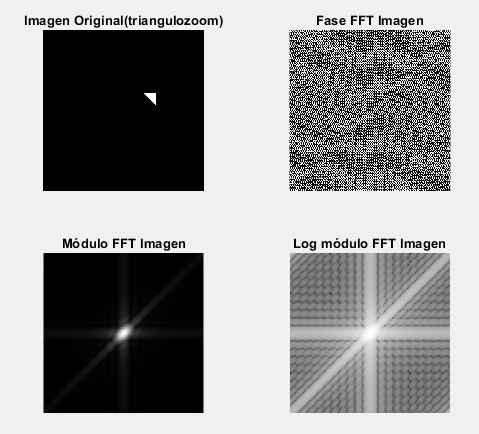
\includegraphics[width=0.4\textwidth]{imagenes/propml}\label{fig:f1}}
  \hfill
  \subfloat[Python]{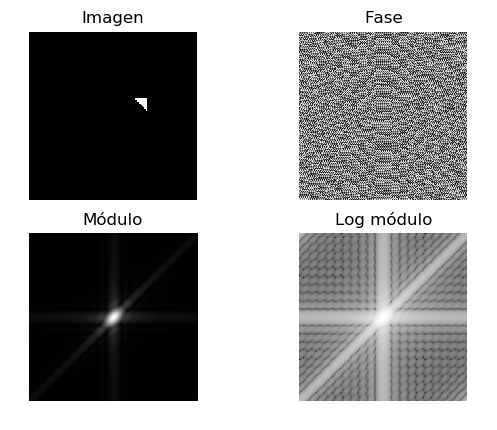
\includegraphics[width=0.4\textwidth]{imagenes/proppy}\label{fig:f2}}
  \caption{Comparativa de resultado en el apartado de propiedades de la transformada}
  \label{zoom}
\end{figure}

Al igual que en la práctica anterior hay una función que viene dada con los materiales de la práctica, en este caso es  \textbf{lpfilter}, una función para generar filtros de tipo Guassiano o ideal. Se recrea con el mismo funcionamiento en Python. A la hora de filtrar, lo que en el espacio era una convolución (ir moviendo una máscara sobre cada pixel) en la frecuencia es una multiplicación punto a punto que se puede realizar con \textbf{numpy.multiply}.\\

El último apartado de filtros paso alto vuelve a usar la función \textbf{lpfilter} para después invertir el filtro de modo que actúe como un filtro paso alto.Para filtrar se repite el mismo proceso[\ref{fpa}].

\begin{figure}[h]
\centering
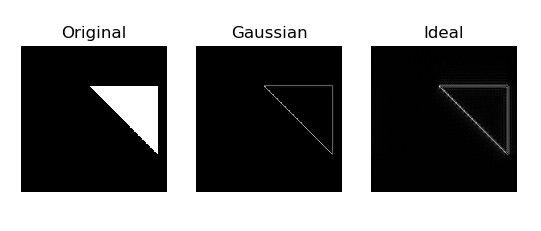
\includegraphics[width=0.6\textwidth]{imagenes/fpa}
\caption{resultados del apartado sobre filtros paso alto}
\label{fpa}
\end{figure}

\subsection{Desarrollo de funciones}

En esta práctica se ha desarrollado una función \textbf{lpfilter} que como se ha mencionado en el apartado anterior genera filtros en frecuencia de dos tipos: Gaussiano e ideal. Como parámetros de entrada recibe el tipo de filtro que se quiere, las medidas del filtro que tienen que coincidir con las de la imagen que se quiere filtrar y D0 que es la apertura del filtro.\\

\section{ Práctica 4: Segmentación de imagen I}
\subsection{Teoría tratada en la práctica}

Esta práctica se centra en entender algunos métodos de segmentación de imágenes usando el ejemplo de una calculadora. En el proceso de segmentar una de las teclas de esta calculadora se van usando varios métodos dados en la teoría de la asignatura.\\

El primero de estos métodos es umbralización usando el histograma, que consiste en elegir un valor como umbral a la hora de convertir una imagen en binaria de forma que queden en primer plano las partes de la imagen que nos interesan. En este caso, las letras de la calculadora.[\ref{thresholding}]\\

\begin{figure}[h]
\centering
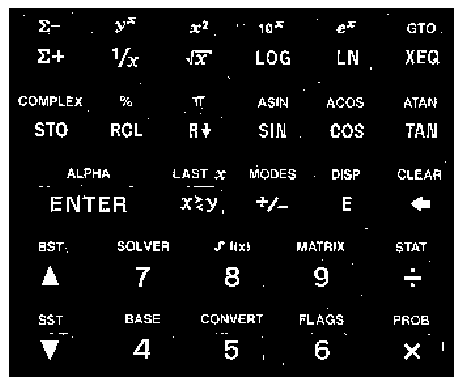
\includegraphics[width=0.6\textwidth]{imagenes/thresholding}
\caption{Imagen tras realizar la umbralización}
\label{thresholding}
\end{figure}
A continuación se explican la segmentación y caracterización de regiones. Segmentación consiste en dividir la imagen en diferentes conjuntos de píxeles llamados regiones, esas regiones forman la capa de segmentación. A cada una de estas regiones se le asigna una etiqueta, la etiqueta 0 se le suele asignar al fondo.\\

Hay varios tipos de segmentación, en este caso se va a usar segmentación binaria que busca grupos conexos de píxeles de primer plano y asigna etiquetas. No todas las regiones van a ser de interés ya que, en muchos casos la umbralización inicial no puede ser perfecta, por ejemplo, por ruido. Para decidir qué regiones son de interés se pueden mirar diferentes características como pueden ser la forma o el tamaño. En este caso se usa el área de la región para decidir cuales son de interés. Tras un proceso de filtrado la imagen queda como se puede ver en la figura \ref{filtersmallareas}\\


\begin{figure}[h]
\centering
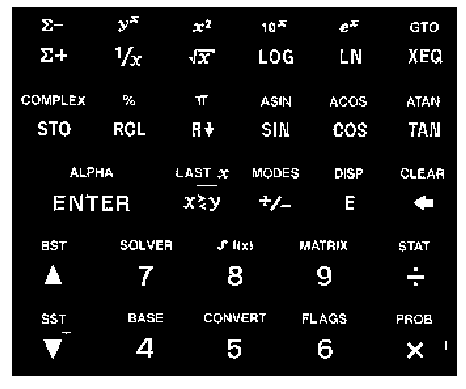
\includegraphics[width=0.6\textwidth]{imagenes/filtersmallareas}
\caption{Resutado de filtrar regiones de area pequeña}
\label{filtersmallareas}
\end{figure}

En este punto, cada letra es una región propia pero, lo que nos interesa segmentar son teclas. Se observa que la distancia entre letras de la misma tecla es muy inferior a la distancia entre letras en diferentes teclas. Para fundir las letras se usa un filtro paso bajo de media. Con esta nueva imagen se repiten todos los procedimientos anteriores hasta que se consigue segmentar solamente la tecla ENTER.[\ref{finp4}]

\begin{figure}[h]
\centering
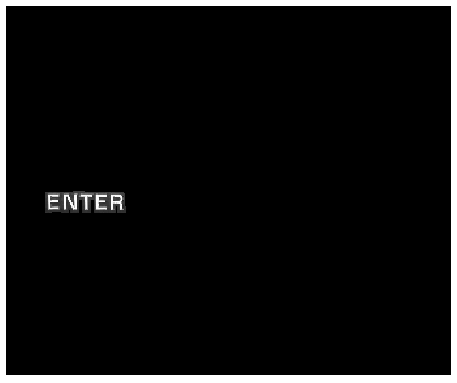
\includegraphics[width=0.6\textwidth]{imagenes/finp4}
\caption{Resutado final de la práctica 4 en Python}
\label{finp4}
\end{figure}


\subsection{Comparativa Matlab vs Python}

En esta práctica hay muy pocas diferencias de Matlab a Python. El apartado de umbralización se mantiene igual, usando las funciones para el histograma y la umbralización que se utilizaron en la práctica 1.\\

En el apartado de segmentación en Pthon nos encontramos con dos opciones, la función de segmentación de OpenCV y la del la librería scikit-image. Se usa la de scikit image ya que funciona de manera mucho más similar a la de Matlab, sobre todo a la hora de conseguir las propiedades de las etiquetas. En OpenCV la función que devuelve propiedades de etiquetas es muy limitada con muy poca información, mientras que la de Scikit devuelve casi exactas las mismas propiedades que el equivalente en MatLab.\\


 Se usan dos funciones para la segmentación y la caracterización de regiones. La primera es \textbf{bwlabel} en Matlab, \textbf{bwlabel} en scikit,  que crea las regiones con píxeles vecinos y devuelve una matriz del tamaño de la imagen original en la que a cada pixel se le ha asignado un número de acuerdo a su región, esta matriz es la capa de etiquetas. La segunda función es \textbf{regionprops} , se mantiene el mismo nombre en ambas versionaes, que recibe de entrada la capa de etiquetas y devuelve medidas de algunas características de la capa de etiquetas, por ejemplo, el área de cada región, la excentricidad o la posicion de los píxeles extremos de cada región.\\

La mayor diferencia entre label en matlab y scikit es el tratamiento de los píxeles de fondo. Matlab trata todo pixel de intensidad 0 como una única etiqueta de valor 0, mientras que scikit aunque en la imagen etiquetada pone los píxeles negros con la etiqueta 0 no lo cuenta como una etiqueta, por lo que por ejemplo en regionprops no tenemos la opción de recibir datos sobre los pñixeles de fond. A la función se le puede indicar que etiquete los píxeles negros pero no funciona igual que matlab, ya que los trata como una etiqueta más, es decir, cuneta como etiquetas diferentes los píxeles negros no conexos. Esto no supone ningún problema en la realización de esta práctica excepto una ligera incomodidad ya que en el array devuelto por \textbf{regionprops} no coinciden los índices con el número de etiqueta en la imagen etiquetada, hay que sumarle uno al índice.

Para representar la capa de etiquetas en color Matlab tiene una función dedicada, mientras que en Python se puede usar cualquiera de los mapas de color disponibles de Matplotlib que generan el mismo efecto. En este caso se usa 'nipy-special' porque mantiene el fondo de color negro. [\ref{color}]\\

El resto de la práctica usa la función de filtrado de media de la práctica 2 y repite los mismos pasos de los apartados anteriores.

\begin{figure}[h]
\centering
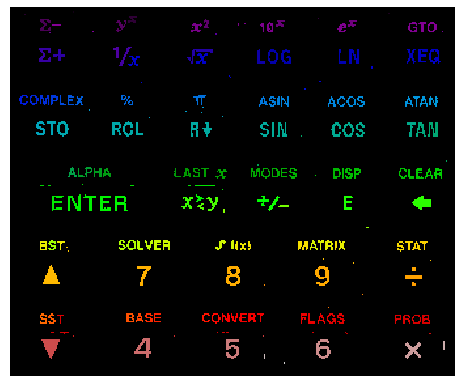
\includegraphics[width=0.6\textwidth]{imagenes/color}
\caption{Capa de etiquetas representada usando 'nipy-special'}
\label{color}
\end{figure}


\section{ Práctica 5: Segmentación de imagen II}
\subsection{Teoría tratada en la práctica}

Esta práctica continúa el tema de la práctica anterior. Intenta segmentar una imagen, en este caso es la figura de un pájaro. Para realizar este proceso de segmentación se va a usar aprendizaje de máquina Kmedias.\\

Usa un sistema de ensayo/error con el objetivo de que el alumno entienda que no todos los métodos funcionan igual para todas las imágenes porque cada imagen tiene unas caractericticas diferentes.\\

El primer método que se intenta para segmentar la imagen es el utilizado en la práctica anterior: umbralización. Al ver el histograma de la imagen del Cormorán queda claro que la umbralización no va a ser posible ya que, no hay una distinción tan clara de tonos como en la imagen de la calculadora.\\

El siguiente método que se usa es el algoritmo K-medias aplicado sobre la imagen en RGB. Cogemos una descripción sencilla del funcionamiento de K-medias de la universidad de Oviedo: "K-means es un algoritmo de clasificación no supervisada (clusterización) que agrupa objetos en k grupos basándose en sus características. El agrupamiento se realiza minimizando la suma de distancias entre cada objeto y el centroide de su grupo o cluster. Se suele usar la distancia cuadrática."[Bibliografía]\\

La característica sobre la que vamos a agrupar estos datos es el color, en este caso se ordenan en una gráfica 3D donde cada eje es una componente de color en RGB[\ref{cormoranrgb}].\\

\begin{figure}[h]
\centering
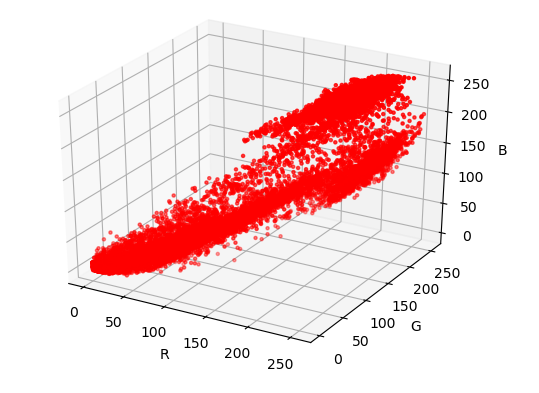
\includegraphics[width=0.6\textwidth]{imagenes/cormoranrgb}
\caption{Representación de los píxeles de la imagen en gráfico 3D}
\label{cormoranrgb}
\end{figure}

 Se decide usar 3 centroides ya que son los colores principales que se aprecian en la imagen (azul para el mar y cielo, amarillo para el tronco y marrón para el pájaro).\\

\begin{figure}[h]
\centering
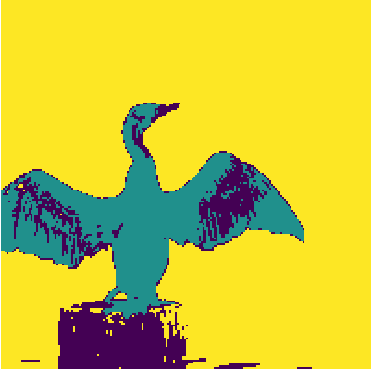
\includegraphics[width=0.6\textwidth]{imagenes/segmentacionrgb}
\caption{Resultado de realizar la segmentación K-medias sobre RGB}
\label{segmentacionrgb}
\end{figure}

En la figura \ref{segmentacionrgb} se ve el resultado de la segmentación, se puede apreciar que tiene varios fallos, por ejemplo, gran parte de las alas del pájaro se han segmentado en el grupo asignado al tronco. Esto se considera sobresegmentación.\\

Para solucionar el problema anterior se prueba un nuevo método, vuelve a usar K-medias, pero en lugar  de organizar los datos en el espacio de color RGB se va a usar Lab. Lab es un espacio de color con tres componentes, la componente L indica la luminancia y las componentes a y b el tono de color.\\

En este ejercicio vamos a usar solamente las componentes ab ya que estamos tratando con tonos muy distintos y la luminancia no es tan relevante. Esto además simplifica los cálculos porque pasamos de usar 3 características a 2 [\ref{cormoranlab}].\\

\begin{figure}[h]
\centering
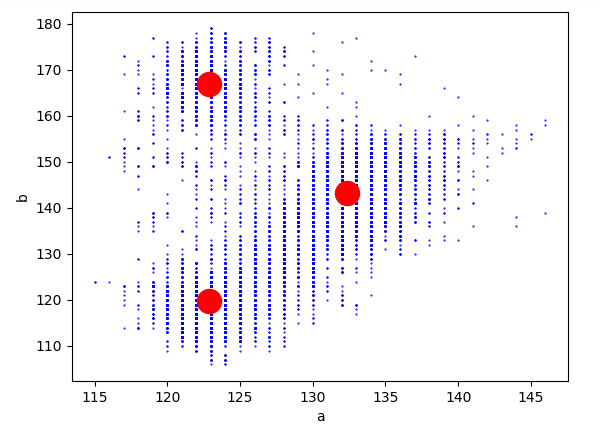
\includegraphics[width=0.6\textwidth]{imagenes/cormoranlab}
\caption{Representación de los píxeles de la imagen en gráfico con ejes a y b}
\label{cormoranlab}
\end{figure}

El resultado vuelve a tener problemas, esto se debe a que los valores de a y b no están estandarizados lo que resulta en que una de las características domina sobre la otra. Una vez se estandarizan el resultado es el que se puede ver en la figura \ref{segmentacionlab}\\


\begin{figure}[h]
\centering
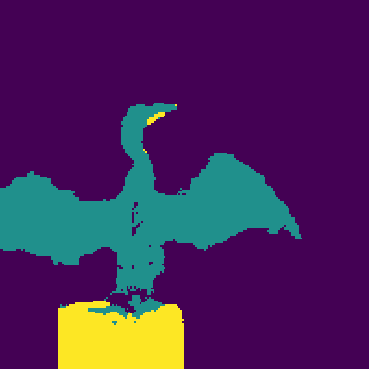
\includegraphics[width=0.6\textwidth]{imagenes/segmentacionlab}
\caption{Resultado de realizar la segmentación K-medias sobre Lab}
\label{segmentacionlab}
\end{figure}

En el cuarto apartado de la práctica se trata la caracterización por textura como alternativa al color. Para realizar esta caracterización se usan diferentes filtros con diferentes resultados en la segmentación también realizada con K-medias.\\

Por último, se prueba a usar varias características de distinta naturaleza, en este caso color y textura, esto resulta en la sobresegmentación de la imagen.[\ref{segmentacionabe}].

\begin{figure}[h]
\centering
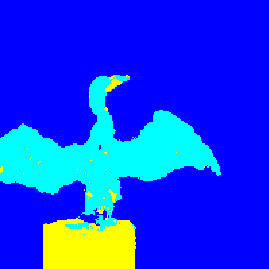
\includegraphics[width=0.6\textwidth]{imagenes/segmentacionabe}
\caption{Resultado de realizar la segmentación K-medias sobre componentes de color y textura}
\label{segmentacionabe}
\end{figure}

\subsection{Comparativa Matlab vs Python}

El primer apartado de la práctica se ha mantenido idéntico ya que no requiere nada más que la función de representación del histograma.\\

En el siguiente apartado lo primero que se pide es recolocar los datos de la imagen de modo que queden en una matriz con 3 columnas y tantas filas como píxeles tiene la imagen. Cada columna contiene los datos de una de las componentes de color RGB, esto nos sirve para la representación en forma de scatter plot. Para convertir una matriz de dos dimensiones en un vector Numpy tiene la función de \textbf{reshape}. \\

Para aplicar kmedias vamos a usar la clase \textbf{Kmeans} de la biblioteca Scikit-learn. Primero se inicializa la clase indicando el número de centroides. Después se llama a la función \textbf{fit\_predict} con nuestra matriz de datos como parámetro, esta función es la que ejecuta el algoritmo, por defecto se realizan un máximo de 10 iteraciones. En el atributo cluste\_centers se guarda la posición final de los centroides, y en labels la capa de etiquetas que es una matriz con la misma forma que la matriz de datos. EL resultado de esta apartado es idéntico al de Matlab. \\

Para representar la capa de etiquetas hay que realizar las transformaciones inversas a las del inicio del apartado. En la figura \ref{comprgb} se puede ver las capas de etiquetas obtenidas en Matlab y Python. \\

\begin{figure}[!tbp]
  \centering
  \subfloat[Matlab]{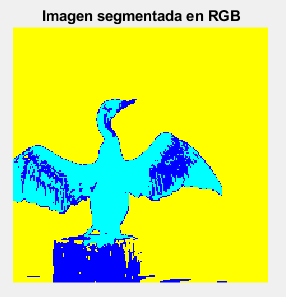
\includegraphics[width=0.4\textwidth]{imagenes/segmentacionrgbml}\label{fig:f1}}
  \hfill
  \subfloat[Python]{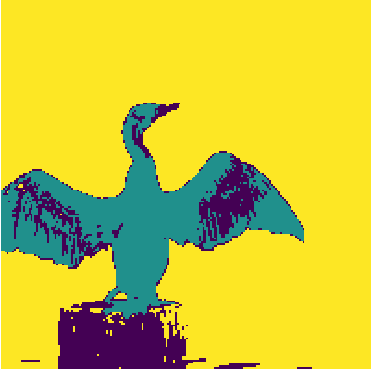
\includegraphics[width=0.4\textwidth]{imagenes/segmentacionrgb}\label{fig:f2}}
  \caption{Comparativa de resultado en la capa de etiquetas}
  \label{comprgb}
\end{figure}

Una diferencia en el apartado sobre el espacio de color LAB es la función usada para cambiar de espacio de color. En la práctica original la función viene dada con el enunciado de la práctica ya que no está implementada en Matlab. En OpenCV la función \textbf{CVTcolor} si que permite pasar de RGB a LAB.\\

En este apartado se pide la normalización de las variables, la secuencia de código necesaria viene dada en el enunciado, esto se ha replicado en el cuadernillo de Jupyter modificando el código para funcionar en Pyhthon.\\

El apartado sobre texturas es el que más cambios ha requerido ya que, las funciones de filtro de textura disponibles en Matlab no existen en OpenCV y han tenido que ser recreadas, lo resultados son idénticos. En figura \ref{entropyfilt} se puede ver la comparativa de aplicar el filtro de entrpía en Matlab y Python.

\begin{figure}[!tbp]
  \centering
  \subfloat[Matlab]{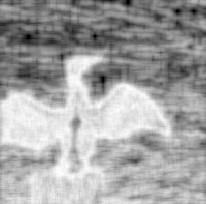
\includegraphics[width=0.4\textwidth]{imagenes/entropyfiltml}\label{fig:f1}}
  \hfill
  \subfloat[Python]{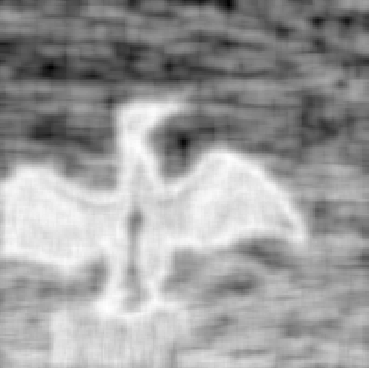
\includegraphics[width=0.4\textwidth]{imagenes/entropyfiltpy}\label{fig:f2}}
  \caption{Comparativa de resultados de aplicar el filtro de entropía}
  \label{entropyfilt}
\end{figure}


\subsection{Desarrollo de funciones}

En este ejercicio se desarrollan 3 funciones nuevas:
\begin{itemize}
	\item \textbf{ stdfilt}: esta función devuelve la imagen filtrada acorde a su variación estándar. Funciona de una manera similar a un filtro de media, con una máscara por defecto de tamaño 3X3 pero, en lugar de hacer la media con los píxeles debajo de la máscara calcula su desviación estándar.
	\item \textbf{ entropyfilt}:
	\item \textbf{rangefilt}:
\end{itemize}



\section{ Práctica 6: Morfología binaria}
\subsection{Teoría tratada en la práctica}

Esta práctica se centra en el uso de la morfología matemática para la segmentación de una imagen. Los operadores morfológicos son una serie de operadores no lineales relacionados con la forma de los objetos en la imagen. Como en las dos prácticas anteriores se va a usar la segmentación de una imagen en concreto para demostrar el funcionamiento de estos operadores. En este caso la imagen es de un circuito impreso, el objetivo es segmentar los 7 chips.\\

Al igual que en la práctica anterior, lo primero que se va a hacer es decidir en qué espacio de color es más cómodo trabajar para esta segmentación. Tras probar en RGB se decide usar HSI, que es un espacio de color que define tono, saturación e intensidad. Mientras que en RGB las tres componentes se veían igual debido a la prominencia de tonos grises en la imagen, en HSI podemos apreciar una gran diferencia entre componentes. En la componente S se ven claramente diferenciados los chips, así que es la que se escoge para continuar el proceso de segmentación.\\

A continuación, se usa la umbralización para trabajar sobre una imagen binaria. Tras este proceso queda algún pixel blanco dentro de los chips que nos interesa eliminar. Se usa un filtro de mediana para homogeneizar la superficie de los chips.\\

En el siguiente apartado, se empiezan a usar operadores morfológicos. Contamos con 4 operadores morfológicos diferentes: erosión, dilatación, apertura y cierre. Para aplicar un operador morfológico se debe usar un elemento estructural. Los operadores morfológicos modifican los píxeles debajo del elemento estructural, la dilatación, por ejemplo, se queda con el máximo valor bajo el elemento estructural, la erosión el mínimo. La apertura y el cierre son elementos compuestos. La apertura es realizar una dilatación tras una erosión y el cierre lo opuesto.[\ref{erosion}]\\

\begin{figure}[h]
\centering
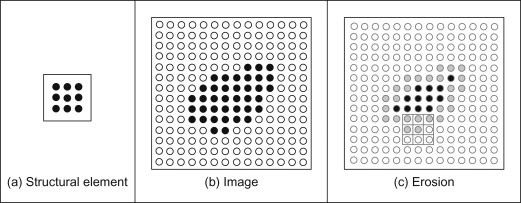
\includegraphics[width=0.6\textwidth]{imagenes/erosion}
\caption{Ejemplo del funcionamiento del operador morfológico erosión}
\label{erosion}
\end{figure}

Para demostrar el efecto de cada uno de estos operadores morfológicos en la práctica se pide que se usen todos sobre la imagen binaria a segmentar probando a cambiar el tamaño del elemento estructural. El objetivo es decidir qué operador morfológico es más apropiado para esta situación y terminar el apartado con una imagen en la que solamente están diferenciados los chips como la de la figura \ref{closing} que es el resultado de aplicar cierre sobre la imagen.\\

\begin{figure}[h]
\centering
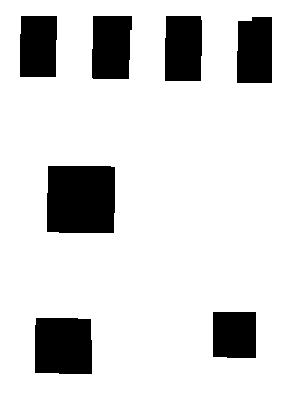
\includegraphics[width=0.6\textwidth]{imagenes/Closing}
\caption{Resultado de aplicar cierre sobre la imagen}
\label{closing} 
\end{figure}

Para realizar la segmentación se invierte la imagen de forma que queden los chips en primer plano. Se segmenta la imagen usando segmentación binaria.\\

La práctica tiene dos apartados más: el primero pide que se use la excentricidad de las etiquetas para separar los chips cuadrados de los rectangulares, esto se hace de la misma manera que en la práctica 4 cuando se discriminaron etiquetas por su área. El segundo y último apartado pide que se usen operadores morfológicos para conseguir los bordes de los chips. Esto se consigue restando el resultado de la dilatación (que expande objetos) menos la erosión ( que reduce el tamaño).\\

\subsection{Comparativa Matlab vs Python}

A la hora de desarrollar el cuadernillo, la primera complicación se encuentra al pasar la imagen de RGB a HSI. En la práctica original, esta función viene dada con el enunciado. En OpenCV tampoco existe esta función por lo que  se tiene que desarrollar de cero. El resultado es idéntico al de Matlab.\\

OpenCV tiene una función con un amplio rango de opciones para operadores morfológicos.  Para la erosión y la apertura se usan funciones dedicadas (\textbf{erode} y \textbf{dilate}), mientras que para la apertura, cierre y otros operadores se usa la misma funcion (\textbf{morphologyEx}) indicando la operación a realizar con un parámetro. Para el elemento estructural se usa una matriz de Numpy.\\

Para diferenciar los chips cuadrados de los rectangulares se mantiene igual ya que la función \textbf{regionprops} de scikit también tiene la característica de xscentricidad.

En el último apartado, que el objetivo es la detección de bordes, se usa un elemento estructural circular. Matlab  tiene una función para crear elementos  estructurantes de diferentes tamaños. OpenCV tiene una equivalente. El operador morfológico para detección de bordes se llama gradiente y la función \textbf{morphologyEx} permite aplicarlo directamente pero, ya que la práctica original pide que se razone cómo se obtendrían los bordes se ha decidido mantener el proceso tal y como estaba. Al final del cuadernillo se menciona la existencia de esta función como información adicional.

\subsection{Desarrollo de funciones}

Este ejercicio ha requerido el desarrollo de una función para cambiar del espacio de color RGB a HSI. Solo tiene un parámetro de entrada y uno de salida, la propia imagen en uint8. No es una función demasiado compleja ya que solamente aplica las fórmulas matemáticas necesarias para esta transformación.[\ref{rgb2hsi}]

\begin{figure}[h]
\centering
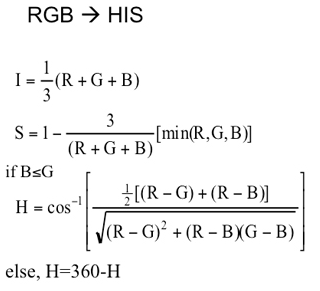
\includegraphics[width=0.6\textwidth]{imagenes/rgb2hsi}
\caption{Fórmulas para pasar de RGB a HSI}
\label{rgb2hsi} 
\end{figure}

\section{ Práctica 7}
\subsection{Teoría tratada en la práctica}

Esta práctica trata el método de segmentación por \emph{Watershed} con marcadores para contar el número de células enteras que hay en una imagen.\emph{ Watershed} es un algoritmo de segmentación basado en morfología matemática que trata la imagen como una serie de desniveles topográficos que forman picos y valles [\ref{watershed}] que se van inundando. Se cogen las depresiones de intensidad como marcadores de los que crece el agua (la etiqueta). El proceso de inundación continúa hasta que toda la imagen está "inundada" y donde se toca el agua de diferentes regiones se forman las lineas de  \emph{Watershed} que limitan las regiones.\\

\begin{figure}[h]
\centering
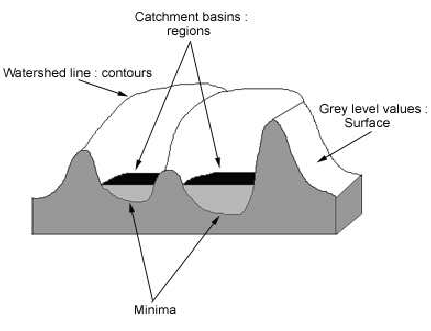
\includegraphics[width=0.6\textwidth]{imagenes/valles}
\caption{Ejemplo de watershed}
\label{watershed} 
\end{figure}

Para que \emph{Watershed} funcione de la manera deseada es necesario extraer los marcadores que indicarán los valles. Primero se extraen los marcadores internos, para ello se trata la imagen en escala de grises con un filtro secuencial alternado que se utiliza para suavizar la imagen. Los filtros secuenciales alternados consisten en realizar de forma secuencial una serie de operaciones morfológicas con diferente elemento estructural, en este caso se alterna entre apertura y cierre con elementos estructurales con forma de disco de radios 1, 2 y 3.\\

A continuación se va a usar reconstrucción que es una operación morfológica que toma una imagen (marker) y la dilata repetidamente hasta que su forma coincide con otra imagen (máscara). Para crear el marcador aplicamos erosión sobre el negativo y usamos el propio negativo como máscara.\\ 

El siguiente paso es extraer los mínimos regionales, un mínimo regional es una región (conjunto de píxeles conexos del mismo nivel) cuyo nivel es inferior al de todos los píxeles que la rodean. Esto devuelve una imagen binaria con más regiones que células en la imagen. Para reducir el número de regiones se usan 3 procesos diferentes:\\

Primero se limpian los bordes, no nos interesan células que no estén enteras ya que podrían aparecer en la siguiente imagen de microscopio y ser contadas dos veces.\\

El siguiente proceso es eliminar las regiones demasiado pequeñas que pueden haber surgido por ruido en la imagen.\\

El último proceso consiste en comparar la posición de nuestras regiones con la posición de los núcleos de las celdas en la imagen original basándonos en que los núcleos aparecen en un color más oscuro, se eliminan todas las regiones cuya posición coincida con un pixel demasiado claro en la imagen original para ser un núcleo.\\

Con eso ya tendríamos los marcadores internos. Para conseguir los marcadores externos (o de fondo) dilatamos la imagen de los marcadores internos para salir de la célula y hacemos una transformada de distancia que, es una operación que devuelve una imagen en escala de grises donde el valor de cada pixel corresponde a la distancia a la que se encuentra de un pixel de primer plano. Los píxeles de primer plano en la transformada de distancia tienen valor 0.\\

Sobre la imagen de la transformada de distancia aplicamos  \emph{Watershed}, los bordes que se forman entre regiones marcan los marcadores externos, siendo los puntos más alejados del nucleo de cada célula.\\

A continuación se crea una imagen que combina los marcadores internos y externos. \\

Para conseguir los bordes reales de las células se vuelve a aplicar  \emph{Watershed}, pero esta vez usando marcadores, como imagen de referencia en lugar de la transformada de distancia se usa el gradiente de la imagen reconstruido de forma que. nuestros marcadores, queden como los únicos mínimos regionales y que los bordes de las células sean los puntos de mayor intensidad de la imagen mientras, que el fondo y los nucleos, al tener menos variación tienen menor intensidad.\\


\subsection{Comparativa Matlab vs Python}

La primera diferencia en esta práctica entre Matlap y Python es la imagen empleada . La imagen original fue sacada de un artículo que no se ha podido localizar y se desconoce su licencia de copyright. Se ha encontrado otra imagen también de celulas muy cercanas las unas a las otras, en este caso de cebolla.\\

El primer apartado se mantiene igual, aplicar un filtro secuencial consiste en realizar repetidas aperturas y cierres sobre la imagen con funciones ya usadas en la práctica anterior.\\

Debido al cambio de imagen algunos de los valores empleados como elemento estructural se han tenido que cambiar, es el caso del elemento estructural usado para la erosión antes de la reconstrucción. Para la reconstrucción se encuentra una función en Scikit-image que funciona exactamente igual al equivalente en Matlab. \textbf{Imreconstruct} en los dos casos recibe una imagen de máscara y una de marcadores.\\

No existe en Python un equivalente a la función \textbf{imregionalmax}. Para conseguir los máximos regionales de una imagen, se ha tenido que programar. La función resultante produce el mismo resultado pero con problemas en cuanto a la velocidad de ejecución.  Si la imagen es muy grande, como es el caso de la imagen en esta práctica, el tiempo de ejecución puede llegar a superar un minuto. La original en Matlab está programada en C lo que la hace más rápida y evita el problema. La otra gran diferencia entre las funciones es que la de Python devuelve regiones más pequeñas que en la de matlab quedan eliminadas. Esto supone añadir un paso más en la práctica para filtrar estas regiones pequeñas usando\textbf{ regionprops} para filtrar por área.\\

A continuación, se eliminan los marcadores que corresponden a las células del borde de la imagen que no están completas, en Matlab se usa la función \textbf{imclearborder}. En Python no hay versión en ninguna librería oficial, pero se ha encontrado una versión en Github subida por el usuario hatamiarash7 que cumple la misma función.\\

Lo siguiente es eliminar los marcadores que no coincidan con un núcleo en la imagen original, en Matlab se usa la función\textbf{ regionprops} con el atributo \emph{mean intensity}, \textbf{regionprops} en scipy-image tiene el mismo atributo con el mismo funcionamiento.\\

Para obtener los marcadores externos se usa la función de dilatar ya mencionada en la práctica anterior y la transformada de distancia, para realizalar Matlab tiene la función \textbf{bwdist} mientras que OpenCV tiene \textbf{distancetransform}. La principal diferencia entre estas dos funciones es que trabajan al revés, la de Matlab devuelve la distancia al punto de primer plano más cercano, mientras que la versión OpenCv devuelve la distancia a 0. Esto se resuelve pasando el negativo de los marcadores a la función en el cuadernillo de Jupyter.\\

A continuación, se aplica \emph{Watershed} sobre esta imagen, en Matlab la función de \textbf{Watershed} recibe como argumento la imagen a segmentar. En Python tenemos dos opciones aunque ninguna funciona exactamente igual que la de Matlab.\\

La primera que se prueba es la versión de OpenCV que se descarta inmediatamente ya que requiere una imagen RGB como primer argumento y la imagen que queremos pasar nosotros es en escala de grises.\\

La segunda opción es la de Scikit-image, también llamada \textbf{Watershed}. Esta si que permite imágenes en escala de grises; la principal diferencia con Matlab es que como segundo argumento pide una imagen binaria de marcadores y si no viene especificada como marcadores se eligen los mínimos locales de la imagen, en la versión de Matlab se cogen los mínimos regionales. En este primer uso de watershed la diferencia no es relevante ya que coinciden los mínimos.\\

 Otra diferencia, ya menor, es que la versión de Matlab automáticamente devuelve las fronteras señaladas en la imagen con un 0 de etiqueta, mientras que en la versión de Scikit-image se tiene que especificar que se requiere etiqueta para las líneas de \emph{Watershed}.\\

Con esto ya tenemos los marcadores tanto internos como externos. A continuación se usa un filtro paso alto para sacar el gradiente del mismo modo que se hizo en la práctica 2. 

Y se vuelve a aplicar  \emph{Watershed}, esta vez la diferencia entre los mínimos si que es relevante así que, en la versión de la práctica en Python, a la función de \textbf{watershed} además de pasarle el gradiente con marcadores como segundo argumento se pasa la imagen binaria de marcadores.\\


\subsection{Desarrollo de funciones}

Para esta práctica se ha tenido que desarrollar la función \textbf{imregionalmax}, que es una función que toma una imagen en escala de grises y devuelve una imagen binaria con los máximos regionales en primer plano. La problemática de esta función es que requiere ir iterando por cada pixel de la imagen y realizando varias operaciones, esto hace que sea imposible de programar directamente en Python ya que el tiempo de ejecución sería demasiado elevado, por ello se han tenido que buscar formas de acortar el proceso lo máximo posible, aunque sigue tardando más que su equivalente en Matlab programado en C.

Para poder ir comprobando el funcionamiento de la función mientras se programaba se creó una imagen simple [\ref{minimos}] en la que se podían ver a primera vista los máximos regoinales .\\


\begin{figure}[h]
\centering
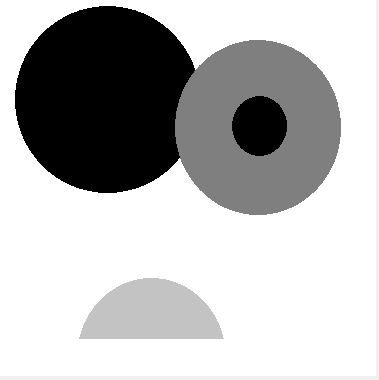
\includegraphics[width=0.6\textwidth]{imagenes/minimos}
\caption{Imagen utilizada en el desarrollo de Imregionalmax}
\label{minimos} 
\end{figure}

Primero se usa la función \textbf{peak\_local\_max}  que devuelve una imagen binaria con los máximos locales en primer plano, a continuación se usa \textbf{connectedcomponents} de OpenCv para etiquetar las regiones de mismo nivel. A continuación se sacan los bordes de las regiones con la función \textbf{findborder}, esto se hace para no ir comparando pixel a pixel, solo se miran los que estén al rededor de un cambio de nivel de intensidad. Aquí es donde se puede ver el primer problema que hay que solucionar, las regiones no son correctas, ya que al usar \textbf{peak\_local\_max} algunos píxeles que son parte de una región pegada a otra de mayor nivel los devuelve como fondo ya que no son máximos locales y esto crea un que da problemas a la hora de comparra píxeles más adelante, para solucionarlo se crea una función \textbf{correctregions} que comprueba si las regiones son correctas o se pueden extender un pixel más que se haya dejado fuera. Se usa esta función entre Connected components y findborders.\\

Ahora recorremos la lista de píxeles borde de región comprobando si los píxeles de su alrededor son del mismo nivel o menores, en el caso de que un pixel sea mayor, esa región no es un máximo regional, por lo que se pone a 0 en la imagen de marcadores y podemos dejar de comprobar el resto de sus bordes. Al final las regiones que quedan son los máximos regionales.


\section{ Práctica 8}
\subsection{Teoría tratada en la práctica}
\subsection{Comparativa Matlab vs Python}
\subsection{Desarrollo de funciones}

\section{ Práctica 9}
\subsection{Teoría tratada en la práctica}
\subsection{Comparativa Matlab vs Python}
\subsection{Desarrollo de funciones}


\chapter{Conclusiones}

\nocite{*}
\printbibliography[heading=bibintoc,title={Bibliography}]

\end{document}